% !TEX TS-program = XeLaTeX
% use the following command: 
% all document files must be coded in UTF-8
\documentclass{textolivre}
% See more information on the repository: https://github.com/leolca/textolivre

% Metadata
\begin{filecontents*}[overwrite]{article.xmpdata}
    \Title{Muito além do relvado: futebol, nacionalismo e redes sociais}
    \Author{Branco Di Fátima \sep Célia Gouveia \sep Sandra Miranda}
    \Language{pt-PT}
    \Keywords{mídia \sep futebol \sep fãs \sep redes sociais \sep Facebook}
    \Journaltitle{Texto Livre}
    \Journalnumber{1983-3652}
    \Volume{14}
    \Issue{3}
    \Firstpage{1}
    \Lastpage{16}
    \Doi{10.35699/1983-3652.2021.29714}

    \setRGBcolorprofile{sRGB_IEC61966-2-1_black_scaled.icc}
            {sRGB_IEC61966-2-1_black_scaled}
            {sRGB IEC61966 v2.1 with black scaling}
            {http://www.color.org}
\end{filecontents*}

\journalname{Texto Livre}
\thevolume{14}
\thenumber{3}
\theyear{2021}
\receiveddate{\DTMdisplaydate{2021}{3}{3}{-1}} % YYYY MM DD
\accepteddate{\DTMdisplaydate{2021}{4}{25}{-1}}
\publisheddate{\DTMdisplaydate{2021}{8}{2}{-1}}
% Corresponding author
\corrauthor{Branco Di Fátima}
% DOI
\articledoi{10.35699/1983-3652.2021.29714}
%\articleid{NNNN} % if the article ID is not the last 5 numbers of its DOI, provide it using \articleid{} commmand
% list of available sesscions in the journal: articles, dossier, reports, essays, reviews, interviews, editorial
\articlesessionname{articles}
% Abbreviated author list for the running footer
\runningauthor{Di Fátima et al}
\sectioneditorname{Daniervelin Pereira}
\layouteditorname{Anna Izabella M. Pereira}


\title{Muito além do relvado: futebol, nacionalismo e redes sociais}
\othertitle{Far beyond the pitch: football, nationalism and social media}
% if there is a third language title, add here:
%\othertitle{Artikelvorlage zur Einreichung beim Texto Livre Journal}

\author[1]{Branco Di Fátima~\orcid{0000-0001-6981-7228}~\thanks{Email: \url{brancodifatima@gmail.com}}}
\author[1]{Célia Gouveia~\orcid{0000-0001-5721-8922}~\thanks{Email: \url{celiamargou@gmail.com}}}
\author[2]{Sandra Miranda~\orcid{0000-0002-5544-5942}~\thanks{Email: \url{smiranda@escs.ipl.pt}}}

\affil[1]{Centro de Investigação e Estudos de Sociologia (CIES), Instituto Universitário de Lisboa (Iscte), Lisboa, Portugal.}
\affil[2]{Escola Superior de Comunicação Social (ESCS), Instituto Politécnico de Lisboa (IPL), Lisboa, Portugal.}


\addbibresource{article.bib}
% use biber instead of bibtex
% $ biber tl-article-template

% set language of the article
\setdefaultlanguage{portuguese}
\setotherlanguage{english}

% for spanish, use:
%\setdefaultlanguage{spanish}
\gappto\captionsspanish{\renewcommand{\tablename}{Tabla}} % use 'Tabla' instead of 'Cuadro'
\AfterEndPreamble{\crefname{table}{tabla}{tablas}\Crefname{table}{Tabla}{Tablas}}

% for languages that use special fonts, you must provide the typeface that will be used
% \setotherlanguage{arabic}
% \newfontfamily\arabicfont[Script=Arabic]{Amiri}
% \newfontfamily\arabicfontsf[Script=Arabic]{Amiri}
% \newfontfamily\arabicfonttt[Script=Arabic]{Amiri}
%
% in the article, to add arabic text use: \textlang{arabic}{ ... }

% to use emoticons in your manuscript
% https://stackoverflow.com/questions/190145/how-to-insert-emoticons-in-latex/57076064
% using font Symbola, which has full support
% the font may be downloaded at:
% https://dn-works.com/ufas/
% add to preamble:
% \newfontfamily\Symbola{Symbola}
% in the text use:
% {\Symbola }

% reference itens in a descriptive list using their labels instead of numbers
% insert the code below in the preambule:
\makeatletter
\let\orgdescriptionlabel\descriptionlabel
\renewcommand*{\descriptionlabel}[1]{%
  \let\orglabel\label
  \let\label\@gobble
  \phantomsection
  \edef\@currentlabel{#1\unskip}%
  \let\label\orglabel
  \orgdescriptionlabel{#1}%
}
\makeatother
%
% in your document, use as illustraded here:
%\begin{description}
%  \item[first\label{itm1}] this is only an example;
%  % ...  add more items
%\end{description}
 

% custom epigraph - BEGIN 
%%% https://tex.stackexchange.com/questions/193178/specific-epigraph-style
\usepackage{epigraph}
\renewcommand\textflush{flushright}
\makeatletter
\newlength\epitextskip
\pretocmd{\@epitext}{\em}{}{}
\apptocmd{\@epitext}{\em}{}{}
\patchcmd{\epigraph}{\@epitext{#1}\\}{\@epitext{#1}\\[\epitextskip]}{}{}
\makeatother
\setlength\epigraphrule{0pt}
\setlength\epitextskip{0.5ex}
\setlength\epigraphwidth{.7\textwidth}
% custom epigraph - END


% if you use multirows in a table, include the multirow package
\usepackage{multirow}
\usepackage[para]{threeparttable}

% add line numbers for submission
%\usepackage{lineno}
%\linenumbers

\begin{document}
\maketitle

\begin{polyabstract}
\begin{abstract}
O artigo analisa as formas como os fãs das seleções de Portugal, Espanha, Marrocos e Irã, o Grupo B do Mundial de Futebol 2018, se envolveram com as suas respectivas páginas oficiais no Facebook e como as páginas se relacionaram com os \emph{stakeholders}. A estratégia adotada assenta numa abordagem quantitativa aos fluxos de dados produzidos, entre 1 de abril de 2017 e 3 de maio de 2018, pelas \emph{fanpages} e por seus utilizadores. A amostra é formada por 3,068 publicações e perto de 11 milhões de interações na rede. Os resultados revelam que os contextos sociais offline potencializam as oportunidades e barreiras para o envolvimento, numa lógica em que o futebol vai muito além do relvado. Os dados apontam que a rede das \emph{fanpages} do Grupo B é formada basicamente por entidades, e só um ator humano integra o TOP 10 dos influenciadores.


\keywords{Mídia \sep Futebol \sep Fãs \sep Redes sociais \sep Facebook}
\end{abstract}

\begin{english}
\begin{abstract}
This paper analyzes how fans of the national teams of Portugal, Spain, Morocco and Iran, the so-called Group B of the 2018 World Cup, got involved with their respective official Facebook pages and how the fanpages related to stakeholders. The strategy adopted is based on a quantitative approach to the data flows produced, between April 1, 2017 and May 3, 2018, by fanpages and their users. The sample consists of 3,068 posts and close to 11 million interactions on the network. Results reveal that offline social contexts highlight the opportunities and the involvement bans, in a logic in which football goes far beyond the pitch. Data show that the network of these pages is basically formed by institutions, and only a human actor is part of the TOP 10 of influencers.

\keywords{Media \sep Football \sep Fans \sep Social media \sep Facebook}
\end{abstract}
\end{english}

% if there is another abstract, insert it here using the same scheme
\end{polyabstract}


\section{Introdução}\label{sec-intro}
É impossível entender completamente as sociedades contemporâneas sem reconhecer o papel do desporto no seu seio. As práticas desportivas ajudaram a construir o tecido cultural de diferentes regiões, localidades e nações ao longo dos tempos \cite{jarvie2006}. Aliás, as ciências sociais destacam as competições coletivas, em especial o futebol, como um espaço privilegiado para expressar identidades comunais \cite{giulianotti2015}. Nas últimas décadas, essas sociedades também passaram a estruturarem-se em torno de um sistema baseado numa linguagem digital, em que a comunicação é desenhada pelo poder das redes \cite{castells2007}.

Talvez por isso, sites como Facebook, Twitter ou YouTube sejam plataformas nas quais os membros de uma determinada comunidade participam na organização, produção e consumo de eventos desportivos. A expressão em rede de símbolos comuns, a história, a equipe e objetivos ou a necessidade de pertença acaba por unir a equipe à comunidade, permitindo utilizar esse espaço virtual para o fortalecimento da identidade \cite{haugh2016}. A comunidade de fãs e a marca da equipe autoidentificam-se por um conjunto de valores partilhados \cite{chadwick2014, newman2017, gouveia2019, lapa2019}.

As atividades dos fãs de desporto nas redes sociais colocam desafios valiosos. As suas interações permitem analisar a formação de comunidades, os interesses partilhados, o papel das federações e a influência dos atores em conjuntura específica. Nesse sentido, este artigo analisa as formas como os fãs das seleções de Portugal, Espanha, Marrocos e Irã – o chamado Grupo B do Mundial de Futebol 2018, na Rússia – se envolveram com suas respectivas páginas oficiais no Facebook e como as \emph{fanpages} se relacionaram com os \emph{stakeholders}.

A estratégia metodológica assenta em uma abordagem quantitativa aos fluxos de dados criados ao longo de um ano, entre os dias 1 de abril de 2017 e 3 de maio de 2018, pelas \emph{fanpages} do Grupo B e pelos seus utilizadores. A amostra é formada por 3,068 publicações e cerca de 11 milhões de interações na rede (gostos, partilhas, comentários, etc.). Esses dados foram extraídos com o Netvizz \cite{rieder2013}, via \emph{Application Programming Interface} (API), e tratados com o pacote estatístico do Gephi. Entre os recursos usados na análise estão o algoritmo \emph{Modularity} – que aplicou cores aos clusters da rede; o layout \emph{Force Atlas 2} – que aproximou as \emph{fanpages} com mais interação dentro dos clusters; e a métrica \emph{Weighted Degree} – que destacou os atores mais influentes \cite{barabasi2016}.

A problematização desses exemplos passou por analisar os dados quantitativos em duas fases. Numa primeira, a comparação entre a atividade das equipes no Facebook. Numa segunda, o exame dos hábitos dos seguidores nas \emph{fanpages}, a partir das interações. Os resultados revelam que os contextos sociais offline potencializam as oportunidades e limitações de envolvimento, numa lógica em que o futebol vai além da mera disputa dentro de quatro linhas. Forças políticas, tecnológicas e culturais, vincadamente diferentes nos países em estudo, podem influenciar os seus fluxos de interação. É possível verificar que a rede de \emph{fanpages} é constituída basicamente por instituições, e apenas um ator humano aparece no TOP 10 dos influenciadores. Deste modo, torna-se difícil separar as atividades sociais offline e online. Fica claro que o desporto, enquanto fenômeno manifesto em rede, espelha características locais e globais.

\section{Local vs global: futebol, nacionalismo e redes sociais}\label{sec-localglobal}
O desporto moderno é culturalmente universal. É praticado e consumido, sob uma forma ou outra, em todo o mundo \cite{wagg2006}. Neste contexto, o futebol está sem dúvidas na linha da frente, tanto na prática quanto no consumo \cite{giulianotti2015}. Em termos gerais, o Mundial de Futebol tem apenas os Jogos Olímpicos como um rival à altura. Por essa razão, os megaeventos desportivos oferecem oportunidades para problematizar as complexas, e às vezes contraditórias, dinâmicas da globalização \cite{gruneau2017, giddens1999}.

Para \textcite{roche2000}, os megaeventos são fenômenos que expressam as atuais tendências do processo de globalização. Por um lado, a hegemonia de culturas e dos mercados. Por outro, as manifestações de identidade que afirmam as especificidades do local e do global. O próprio impacto político-ideológico que os megaeventos alcançam vai muito além do que acontece no terreno de jogo \cite{rowe2003}. O processo de globalização contribuiu ao acrescentar elementos que tornam o desporto cada vez mais multicultural \cite{jenkins2012}, embora não exista razão para crer que o nacionalismo como força cultural caiu em esquecimento \cite{rowe1998}.

A cultura nacional é pensada como algo no qual uma pessoa nasce e cria uma identidade \cite{maguire1993}. Por essa razão, os megaeventos podem ser entendidos como testes de lealdade fundados no chauvinismo cultural, neste caso, desportivo. Há, aliás, razões para acreditar que a nação desportiva assegura a dimensão simbólica, gerando um sentido específico de lealdade. É notória a ação estimuladora dos processos simbólicos de criação da nação, com convites para fazer parte de manifestações de afirmação \cite{frederick2016, marivoet2006}, como o Mundial de Futebol 2018. A nação desportiva é, portanto, mostrada como uma formação profundamente ideológica, cuja artificialidade, isto é, a construção, é igualada só pela unidade de afirmar a sua pureza orgânica \cite{hobsbawm2012}.

Enquanto o futebol proporciona a sensação de pertença \cite{pinheiro2002}, também influencia as emoções quase a nível do fervor religioso \cite{dorsey2016, gouveia2019}. Nas redes sociais, a emoção pode ser transportada de muitas formas, com textos, imagens, infografias, vídeos, etc. Ou seja, a emoção é multimédia. Nesse caso, por exemplo, parece cada vez mais comum a utilização dos \emph{emojis} associados a sentimento \cite{novak2015}, como tristeza ({\fontspec{Symbola}\symbol{"1F613}}), amor ({\fontspec{Symbola}\symbol{"2764}}), felicidade ({\fontspec{Symbola}\symbol{"1F601}}), sofrimento ({\fontspec{Symbola}\symbol{"1F630}}), raiva ({\fontspec{Symbola}\symbol{"1F620}}), surpresa ({\fontspec{Symbola}\symbol{"1F62F}}), etc. O \emph{emoji} permite que o utilizador de redes sociais expresse sentimentos por uma mensagem, sem recorrer a elementos verbais, de maneira rápida, sintética e apelativa, ideal para a construção da narrativa desportiva. Afinal, o desporto sempre foi um meio por onde sentimentos são comunicados \cite{wenner1989}, ainda que com significados muito distintos em cada cultura.

A história do futebol não pode ser compreendida fora dos contextos de desenvolvimento sociocultural das nações. Parafraseando \textcite[p. 658]{claussen2007}, “futebol e sociedade não estão separados pela Grande Muralha da China”. Assim, apesar do rápido crescimento do futebol nos mercados mundiais, há uma variedade considerável de modelos de negócio, caracterizados por forças históricas, culturais, econômicas e políticas locais. É importante notar que as identidades nacionais, por vezes, têm práticas concorrentes. Aliás, a narrativa de cada localidade edifica os significados que influenciam as ações desportivas, inclusive entorno de megaeventos. Eventos como esses estimulam o envolvimento da população, reforçando atos de Estado \cite{marivoet2006}. Equipes tornam-se legítimas representantes de um espaço, com a afirmação territorial e cultural. Este é o caso das seleções que integraram o Grupo B do Mundial 2018.

O Grupo B era formado por países com valores culturais e sociais heterogéneos. De um lado, Portugal e Espanha, com ampla maioria católica, governos democráticos dentro da União Europeia (UE), estruturas de comunicação robustas e tradição consolidada no futebol mundial – 5º e 6º lugares, respectivamente, no ranking de seleções da \textcite{fifa2021}. De outro lado, Irã e Marrocos, com ampla maioria muçulmana, sob governos autoritários, com acesso limitado às TIC e pouca tradição no futebol – 31º e 34º lugares, respectivamente, no ranking da \textcite{fifa2021}. Para entender as diferenças, torna-se necessário fazer um breve itinerário teórico sobre os países em análise, com atenção especial ao contexto histórico-político e a sua relação com o futebol.

Durante décadas, o futebol construiu um espaço público alternativo no Médio Oriente, proporcionando um ambiente para expressar frustrações contra o autoritarismo \cite{dorsey2016}. Na República Islâmica do Irã, Estado teocrático, a popularização do futebol foi historicamente contestada. Os iranianos responderam ao jogo com um cruzamento de curiosidade, por parte da classe proletária, e desaprovação, da pequena-burguesia \cite{fozooni2004}. Os imperativos modernistas do futebol eram um grande desafio para os desportos locais, particularmente o zurkhãneh (atletismo que combina movimentos de ginástica, artes marciais e música). O futebol esteve sempre ligado à política, quer a nível nacional, quer internacional. Esse impulso de modernização, durante a Revolução Constitucional (1905-1911) e reinado do xá Reza Pahlavi (1925-1941), permitiu ao futebol tornar-se em um mecanismo de transferência da lealdade tribal para o governo central \cite{chehabi2002}.

O futebol no Irã continua a ser um importante terreno ideológico \cite{fozooni2004}. Nos últimos anos, tornou-se um espaço privilegiado de contestação social. Para \textcite{dousti2013}, o jogo é uma arena sob pressão, onde facções rivais fazem uma curiosa “guerra por procuração”, já que não há interesse real em declarar hostilidade ao futebol. Algumas formas de secularismo expulsaram a religião das bancadas, reduzindo as demonstrações de poder das forças religiosas que controlam o país. Com isso, a rivalidade entre clubes do interior e da capital alcançou novos patamares, refletindo a antipatia em relação à Teerão como lugar de poder do regime \cite{fozooni2004}. Assim, é comum que os jogos internacionais deem origem a grandes manifestações, com milhares de jovens nas ruas. Os clubes iranianos, com status de semipúblicos, estão cada vez mais procurando financiamento privado para competir no acirrado mercado do Médio Oriente. Os clubes patrocinados, como o Persépolis F.C., adotam lentamente práticas de gestão profissional da marca \cite{chehabi2002}.

No caso de Marrocos, o futebol é o desporto mais popular desde a colonização europeia, no século XIX. Com uma rápida popularização no país, em 1955 foi criada a primeira equipa nacional. A partir daí, lançaram-se campeonatos, construíram-se estádios e o culto à bola afirmou-se como prática social, amplamente partilhada em comunidade. No passado, antes da independência, o futebol era tido como um desporto de palácio. Em 1959, o príncipe Hassan II estabeleceu o Royal Football Club, uma das equipas mais competitivas da liga marroquina. As competições sob patrocínio da família real tornaram-se comuns, com a definição da agenda da Royal Cup. O desporto era considerado uma ferramenta infalível para conter as massas, vender sonhos e ocupar os jovens, numa altura que a “propaganda subversiva” estava muito em voga, sobretudo na vizinha Argélia \cite{el-caid2006}. Desde os primeiros anos do protetorado francês (1912-1956), os estádios eram um lugar privilegiado para mostrar resistência ao poder colonial, apresentar demandas políticas e sociais \cite{alami2018}.

O futebol marroquino tornou-se conhecido a partir do Mundial 1970, no México, com a sua primeira classificação para um torneio internacional, e a partir do Mundial 1986, no México, sendo a primeira seleção africana a passar da fase de grupos \cite{alami2018}. O sucesso no campo desportivo reforçou a coesão nacional contra ameaças internas e externas, sobretudo no conflito contra o Saara Ocidental. Exacerbando uma tendência vista em outros países do Mundo Árabe, Marrocos candidatou-se como sede dos mundiais de 1994, 1998, 2006 e 2026. O país ambiciona recuperar a credibilidade manchada pelas décadas de autocracia, e um megaevento poderia impulsionar a frágil economia nacional \cite{el-caid2006}. Marrocos conquistou a Taça das Nações Africanas (1976) e a Taça das Nações Árabes (2012).

Em Espanha, o futebol dá os primeiros passos com a comunidade britânica, como prática popular entre a classe operária nas companhias inglesas sediadas no país e que já praticavam a modalidade desde 1878. No primeiro terço do século XX, o futebol organizou-se regionalmente e expressou o que são hoje as identidades nos níveis local, provincial e regional \cite{quiroga2013, tunon2012}. Após a Guerra Civil (1936-1939), a ditadura de Franco unificou o futebol e promoveu a seleção nacional, com centralidade do Real Madrid \cite{tunon2012}. Em contraste com o regime, o nacionalismo catalão foi contra-hegemônico e utilizou o F.C. Barcelona para promover as narrativas catalãs. As décadas de 1960 e de 1970 são muitas vezes consideradas como o período em que o futebol atuou como catalisador das identidades. Os clubes representam as culturas regionais, e o campeonato nacional é um campo simbólico dessa afirmação \cite{quiroga2013}.

A Espanha é um dos maiores expoentes do futebol mundial, quer em termos de clubes, quer em termos de seleção. Como desporto mais praticado no país, o futebol exerce grande impacto social, gera paixões, reconstrói identidades e desenvolve sentimentos profundos de adesão \cite{tunon2012}. O futebol foi, a princípio, estabelecido como uma esfera pública ritualizada, que construiu representações do nacional e do regional. A Real Federación Española de Fútbol é uma das organizações fundadoras da FIFA e com mais participações em mundiais. Entre os títulos conquistados estão o Mundial 2010 e os campeonatos europeus de 1964, 2008 e 2012. Em 1982, a Espanha organizou o Mundial. Esse evento é um exemplo dos processos de mercantilização do desporto. Foi transmitido ao maior público da história da televisão até a data e atraiu um número sem precedentes de patrocinadores \cite{llopis_goig2016}.

Em Portugal, o futebol é desporto nacional. A configuração desportiva no território luso constitui um espaço potenciador de uma forte identificação com as equipas e a seleção nacional \cite{marivoet2006}. A modalidade deu-se a conhecer por influência da alta burguesia ligada aos ingleses então residentes no país, na transição dos séculos XIX e XX. A primeira partida envolvendo portugueses deu-se ainda em 1888, em Lisboa, organizada pela aristocracia que tinha contactos com os ingleses e filhos a estudar em Inglaterra \cite{pinheiro2002}. No início do século XX surge o primeiro clube de base claramente popular. Em 1922, foi criado um campeonato nacional, organizado pela União Portuguesa de Futebol (UPF), com forte apelo ao associativismo. Durante o Estado Novo (1933-1974), o desporto foi utilizado para manipular os processos identitários, como instrumento de afirmação do orgulho pátrio e multirracialidade do Império \cite{domingos2006}. O culto à bola também alavancou a ideia de unidade nacional entre as populações do continente e do ultramar.

Em 2004, Portugal organizou o \emph{European Football Championship} e foi o vice-campeão. O megaevento teve grande impacto social e criou um marco simbólico no orgulho nacional. A seleção portuguesa tem atualmente presença constante nos lugares de topo do ranking da \textcite{fifa2021}. Além de ter ficado em 4º lugar no Mundial 2006, na Alemanha, chegou às meias-finais do Euro 2000 e Euro 2012. O país sagrou-se Campeão da Europa em 2016, momento mais alto do futebol nacional. De regresso a Lisboa, a seleção percorreu as ruas e foi recebida com euforia por milhares de adeptos. Se, no passado, a nação usou a modalidade para se legitimar, agora, é a bola que se impõe à política. A futebolização da sociedade tornou-se um fenômeno integrado numa cultura popular \cite{pinheiro2002}.

Nas últimas décadas, Irão, Marrocos, Espanha e Portugal também passaram a estruturarem-se num sistema baseado em linguagem digital, e o quotidiano é desenhado pela lógica das redes \cite{castells2007}. Nesse novo sistema, capaz de incluir todas as expressões culturais, os fãs utilizam os meios de informação e de comunicação para seguir os jogos, discutir os lances mais polêmicos, criar comunidades baseadas em afiliações e consumir notícias sobre equipas, jogadores e entidades. Os fãs nunca souberam tanto sobre atletas e clubes, pelo \emph{feed} do Twitter e Facebook, vídeos no YouTube, textos de blogs pessoais e portais especializados. Produtor e consumidor, adeptos e jogadores, estão cada vez mais articulados numa relação mediada pelas redes. Assim, quanto mais os membros da comunidade interagem com a organização, maior é a probabilidade de se considerarem parte dela \cite{ahn2014, williams2012}.

Quando os seguidores das páginas de atletas, clubes e entidades se situam num universo culturalmente semelhante, eles assumem especial importância por estabelecer um leque diverso de relações – de mercado, de poder, de cooperação, etc. Não é de estranhar, por isso, que muitas das contas de Twitter, Facebook ou YouTube com mais seguidores pertençam a atletas, clubes e entidades desportivas \cite{clavio2010}. Essas plataformas lançam desafios na tomada de decisão em grupo, porque reúnem um grande número de utilizadores de diferentes origens culturais, níveis de conhecimento, envolvimento e prestígio \cite{leen2018}. Esse é o caso dos \emph{lead users}, importantes frente às forças da globalização que têm conduzido o futebol nas últimas décadas \cite{hambrick2012, raaij1997}).

A internet tornou possível uma audiência global. Os fãs de futebol fazem hoje parte de uma comunidade mais alargada, com adeptos distribuídos por múltiplos países. Porém, isso não quer dizer que haja homogeneidade das expressões culturais na audiência global. Para \textcite{miller2001}, a nação cultural como potência demonstra que a audiência global dos megaeventos desportivos é mitológica, já que o global é abstrato e os membros da audiência são interpelados em termos das suas identidades assumidas. Sendo assim, “o espaço e o tempo são comprimidos pela tecnologia, fluxos de informação e relações comerciais e de poder, permitindo que as ações distantes tenham maior significado ao nível local” \cite[p. 131]{miller2001}. O Facebook é um dos exemplos mais pertinentes da cultura desportiva dos mídias globais. Mas, será que a utilização desta plataforma reproduz um padrão social semelhante no mundo inteiro? Os fãs das seleções do Grupo B podem ajudar a responder à pergunta, porque têm características próprias de vivenciar o mundo digital, em larga medida, influenciadas por seu passado colonial ou pelas forças modulares do imperialismo \cite{hobsbawm2003, kamrava2012}.

A sociedade é que dá forma às tecnologias, conforme os valores, as necessidades e os interesses dos seus utilizadores \cite{castells2009, castells2007}. O ciberespaço permite, com efeito, o estabelecimento de redes de comunicação entre indivíduos que pensam, sentem e falam em diferentes idiomas. A capacidade de utilização das tecnologias, bem como o acesso a fluxos de informação que cruzam o mundo, definem, na atualidade, as condições de existência de cada país e de cada região na Sociedade da Informação \cite{macedo2011}. É deste modo que o poder das organizações e dos indivíduos fica dependente do posicionamento frente às redes digitais e ao livre acesso a dados. Irão, Marrocos, Espanha e Portugal lidam com paradigmas diferentes (Quadro \ref{tab1}), num momento que os mecanismos de inclusão e de exclusão também são moldados pelas tecnologias \cite{lapa2019}.

\begin{table}[htpb]
\centering
\begin{threeparttable}
\caption{Indicadores de liberdade e acesso às tecnologias do Grupo B
}
\label{tab1}
\begin{tabular}{lllll}
\toprule
Indicador & Portugal & Espanha & Irão & Marrocos
\\
\midrule
World Press Freedom Index\tnote{a} & 12° & 29° & 170° & 135°
\\
Democracy Index\tnote{b} & 26° & 22° & 152° & 96°
\\
Human Freedom Index\tnote{c} & 26° & 29° & 117° & 158°
\\
Penetração da Internet\tnote{d} & 78,2\% & 92,5\% & 76,0\% & 61,6\%
\\
Penetração do Facebook\tnote{d} & 72,4\% & 53,3\% & 63,8\% & 66,5\%
\\
\bottomrule
\end{tabular}
\centering
\source{
\begin{tablenotes}
\item[a] \textcite{reporteres2019};
\item[b] Economist Intelligence Unit (2021);
\item[c] \textcite{cato2020};
\item[d] \textcite{internet2018, internet2019a, internet2019b}.
\end{tablenotes}
}
\end{threeparttable}
\end{table}

A internet foi introduzida no Irão em 1993, quando o regime xiita decidiu estabelecer a Rede Nacional de Dados (NIN). Nomeada de IranPack, a rede está sob tutela da Companhia de Telecomunicações do Irão. Desde então, é utilizada pelo cidadão iraniano médio, sobretudo para o entretenimento \cite{shoraka2002}. De acordo com a \textcite{internet2018}, 76,0\% da população têm acesso à internet e, 63,8\% deles, perfil no Facebook. Em contrapartida, a censura de sites e o bloqueio de redes sociais são um fenómeno presente, num dos países mais ativos da blogosfera \cite{sreberny2010}. Contudo, o processo de filtragem na internet não é simples e seria impossível sem respaldo das operadoras instaladas no Irão. Com o rígido controlo estatal do espaço público, as redes introduziram novas formas de participação política e protestos \cite{rahimi2011, di_fatima2019}. Hoje, o país ocupa a 170ª posição do \emph{World Press Freedom Index} \cite{reporteres2019}.

Marrocos disponibilizou os serviços de acesso à internet em 1995, enquanto importantes reformas eram realizadas no setor das telecomunicações \cite{clark1998}. À época, a rede era administrada pelo \emph{Office National des Postes et Télécommunications} (ONPT). Desde então, a infraestrutura da internet teve rápido crescimento, e as atividades de comunicação e de entretenimento são as mais realizadas pelo utilizador comum \cite{constant2011}. De acordo com a \textcite{internet2019a}, 61,6\% da população têm acesso à rede e, 66,5\% deles, perfil no Facebook. Com a eclosão dos protestos da Primavera Árabe, em 2011, as redes sociais criaram um espaço para o debate de alternativas políticas. A monarquia avançou com mudanças na legislação e fortaleceu o seu aparato de vigilância digital, com inúmeros ativistas ameaçados e presos por atuações online \cite{zaid2016}. O país surge no 135º lugar do \emph{World Press Freedom Index} \cite{reporteres2019}.

A internet foi introduzida em Espanha em meados de 1990, num projeto experimental chamado RedIRIS, sobretudo no âmbito acadêmico. Desde então, a rede é usada por espanhóis sobretudo para buscar informações noticiosas e atividades de entretenimento, com uma forte presença dos dispositivos móveis na dieta mediática \cite{aimc2019}. De acordo com os dados da \textcite{internet2019b}, 92,5\% da população têm acesso à rede e, 53,3\% deles, perfil no Facebook. As redes sociais têm desempenhado um papel importante para a amplificação dos espaços de debate \cite{camposdominguez2017}, principalmente no rescaldo da crise econômica de 2008. Ferramentas de censura também têm sido utilizadas nos últimos anos, pelo Judiciário, como no bloqueio dos sites sobre o referendo de independência da Catalunha \cite{poblet2018}. O país ocupa a 29ª posição do \emph{World Press Freedom Index} \cite{reporteres2019}.

Portugal faz parte do grupo dos 40 primeiros países a conectarem-se à internet, em 1991, a partir da Universidade de Lisboa e da Universidade do Minho \cite{souza2017}. Na época, o serviço era oferecido pelo \emph{Portuguese Unix Users Group} (PUUG). A partir de então, a internet passou a configurar a dieta mediática nacional, principalmente para o consumo de informações, atividades de entretenimento e comunicação \cite{cardoso2006}. De acordo com dados da \textcite{internet2019b}, 78,2\% da população têm acesso à rede e, 72,4\% deles, perfil no Facebook. Nos últimos anos, praticamente todos os partidos deram início à utilização da internet, com influência das redes no voto \cite{magalhaes2008} e na visibilidade de forças políticas associadas à extrema-direita \cite{palma2021}. O país está no 12º lugar do \emph{World Press Freedom Index} \cite{reporteres2019}.

\section{Abordagem metodológica}\label{sec-abordagem}
A estratégia metodológica utilizada assenta numa abordagem quantitativa aos fluxos de informação produzidos, entre 1 de abril de 2017 e 3 de maio de 2018, nas \emph{fanpages} das seleções de Irão, Marrocos, Espanha e Portugal, o Grupo B do Mundial FIFA 2018, na Rússia. A amostra é constituída por 3,068 publicações (fotos, vídeos, textos, etc) das páginas e cerca de 11 milhões de interações (gostos, partilhas, comentários, \emph{emojis}, etc) dos utilizadores nas \emph{fanpages}.

A extração dos dados utilizou o Netvizz, uma aplicação do Facebook desenvolvida pelo professor Bernhard Rieder, da Universidade de Amesterdão, na Holanda. O Netvizz conecta-se à \emph{Application Programming Interface} (API) da rede social e, a partir do número de identificação das \emph{fanpages}, recolhe os metadados das publicações, como o tipo de mensagem, data e hora de publicação, número de partilhas, links, etc. \cite{rieder2013}. Para o estudo, a opção escolhida foi a \emph{Page Post}, delimitada pelo ano que antecedeu o Mundial 2018. Por motivos associados às políticas de acesso à API do Facebook, o Netvizz foi descontinuado \cite{rieder2019}.

A análise assenta numa categorização dos conteúdos veiculados e dos tipos de interação dos utilizadores com essas publicações, com o auxílio do pacote estatístico do Gephi. Entre os recursos utilizados estão o algoritmo \emph{Modularity} – que aplica cores aos clusters da rede; o layout \emph{Force Atlas 2} – que aproxima as \emph{fanpages} com mais interação dentro desses clusters; e a métrica de \emph{Weighted Degree} – que destaca os atores mais influentes \cite{barabasi2016}.

Especialmente para a soma de envolvimento dos fãs com as páginas das seleções, usou-se o cálculo de \emph{engagement} do Facebook, isto é, a fórmula: ‘comentários + gostos + partilhas ÷ pelo número de seguidores x 100’ \cite{vadivu2015}. A contagem permite ponderar o número total de interações pelo alcance potencial das \emph{fanpages}, medido pelo número de seguidores. Na época da extração dos dados, Portugal e Espanha já tinham páginas com mais 3,5 milhões de seguidores cada, ao passo que Marrocos e Irão contavam com menos de 300 mil cada. Os dados de envolvimento são cruzados com o calendário de compromissos das seleções, com o objetivo de perceber a influência dos jogos na interação dos fãs.

O estudo segue o caminho da análise comparada entre \emph{fanpages}, enquanto manifestação institucional do trabalho das equipas de comunicação do Grupo B, e das relações sociais criadas pelos fãs com um conjunto delimitado de publicações. A problematização dos exemplos passou pela análise dos dados em duas etapas. Em uma primeira fase, a comparação entre as atividades das equipas. Em uma segunda, o exame dos hábitos dos seguidores nas páginas. Dessa maneira, os dados sugerem como os fãs das seleções se envolveram com suas respetivas \emph{fanpages}.

\section{Resultados}\label{sec-resultados}
No ano que antecedeu o Mundial 2018, na Rússia, as seleções do Grupo B veicularam, em conjunto, 3,068 \emph{posts} nas suas respetivas páginas de Facebook. A \Cref{fig1} mostra que a Espanha liderou o ranking, com 1,305 publicações (42,5\%), entre 1 de abril de 2017 e 3 de maio de 2018, seguida por Portugal (776) e Marrocos (769), com frequências praticamente idênticas ao longo do tempo, e pelo Irão (218), bem abaixo da média.

\begin{figure}[htbp]
 \centering
 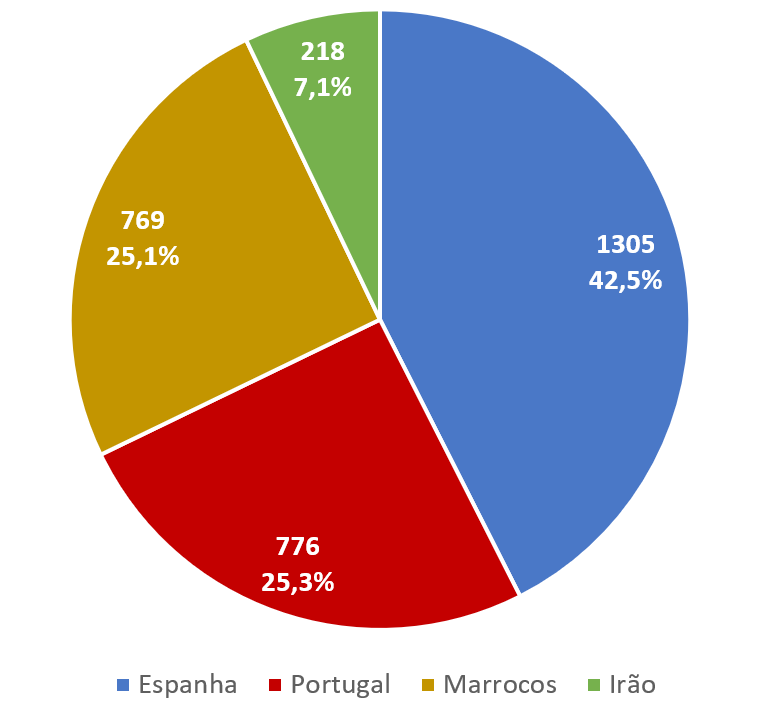
\includegraphics[width=0.7\textwidth]{figure01.png}
 \caption{Publicações do Grupo B no Facebook (n = 3,068).}
 \label{fig1}
 \source{Facebook Graph API}
\end{figure}

O desempenho iraniano pode ser explicado por longos períodos sem atividade na página, com dois intervalos de mais de 60 dias cada, em que não foram veiculados conteúdos da seleção (abril e maio de 2017 | julho e agosto de 2017). Como a censura à internet é uma realidade no país \cite{sreberny2010}, é presumível que esses tenham sido meses de bloqueio das redes sociais, em prejuízo à interação dos fãs da seleção nacional. Mas independentemente do interdito, o Quadro 2 revela a preferência dessas páginas pela publicação de fotos (1,508), seguidas pelos vídeos (836), links (698), eventos (15) e status (14).

\begin{table}[htpb]
\caption{Tipos de publicação do Grupo B no Facebook (\%)}
\label{tbl02}
\centering
\begin{tabular}{lllll}
\toprule
& Irão & Marrocos & Espanha & Portugal
\\
\midrule
Fotos & 88,1 & 79,5 & 17,6 & 61,2
\\
Vídeos & 3,2 & 12,9 & 34,0 & 36,9
\\
Links & 6,4 & 6,1 & 48,4 & 0,4
\\
Eventos & 0,0 & 0,4 & 0,0 & 1,5
\\
Status & 2,3 & 1,2 & 0,0 & 0,0
\\
\bottomrule
\end{tabular}
\centering
\source{Facebook Graph API}
\end{table}

Essa é uma tendência comum a quase todas as equipas do grupo, com destaque para a veiculação de retratos dos atletas, do saldo dos jogos, de lances das partidas, etc. Na divisão proporcional dos resultados, o Irão tem a \emph{fanpage} que mais publica fotografias, com 88,1\% de todo o seu conteúdo, à frente de Marrocos (79,5\%), Portugal (61,2\%) e Espanha (17,6\%), alimentando dessa forma a página com menor diversidade do grupo. Já os espanhóis mantêm o maior equilíbrio na hora de veicular os conteúdos, com a partilha mais igualitária de links (48,4\%) e vídeos (34,0\%).

O Grupo B é um exemplo do poder de conexão das redes. As páginas analisadas seguem outras 194 \emph{fanpages} e estabelecem, juntas, 681 ligações, ou, caminhos para o fluxo informativo. Isto acontece porque quando uma página segue outra, as informações veiculadas surgem no seu \emph{news feed} e podem ser um elemento de influência na tomada de decisão. Seguir muitas \emph{fanpages} também representa a construção de uma base de apoio online, solidária, já que as páginas podem partilhar uma visão de mundo. Neste sentido, Portugal é a seleção que mais segue outras páginas (71), à frente do Irão (62), Espanha (55) e Marrocos (14). A \Cref{fig2} mostra os tipos de página, segundo categorização do Facebook, com mais conexões.

\begin{figure}[htbp]
 \centering
 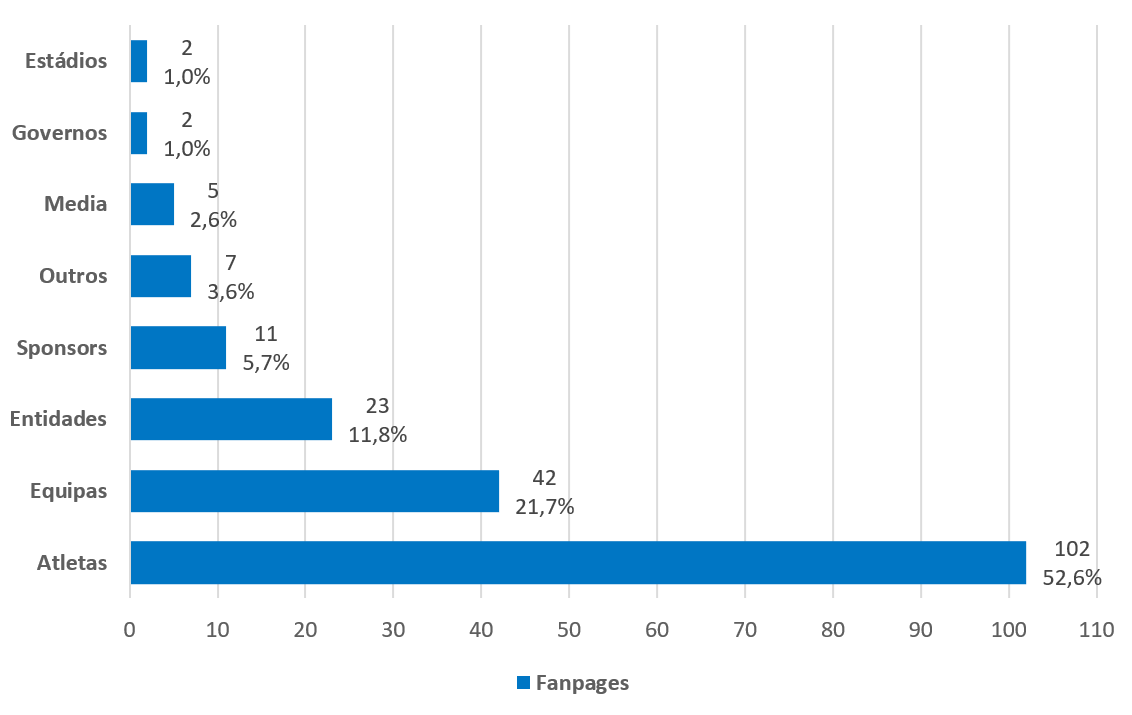
\includegraphics[width=0.85\textwidth]{figure02.png}
 \caption{Páginas seguidas pelo Grupo B no Facebook (n = 194).}
 \label{fig2}
 \source{Facebook Graph API}
\end{figure}

Os atletas profissionais, sobretudo àqueles que jogam pelas seleções estudadas, têm as páginas mais seguidas do Grupo B (52,6\%), como Ashkan Dejagah (Irão) ou Cristiano Ronaldo (Portugal). Clubes e seleções de outros países têm um peso significativo no total (21,7\%), como as equipas nacionais do Brasil, Alemanha ou Estados Unidos. As \emph{fanpages} de entidades surgem em terceiro lugar (11,8\%), encabeçadas por organizações desportivas do futebol, como a FIFA, UEFA ou CAF. Surpreendentemente, os patrocinadores têm um peso menor do que se poderia esperar (5,7\%), com destaque para uma combinação de empresas de diferentes setores (aéreas, eletrónicos, alimentação, energia, comunicações, etc), e não só as ligadas ao desporto (Adidas, Nike, etc). Já nos últimos lugares estão os órgãos de comunicação (2,6\%), páginas de governo (1,0\%) e de estádios (1,0\%).

Como \emph{stakeholders} das seleções e protagonistas do mercado global, essas organizações também interagiram, ao longo do ano em estudo, no Facebook. A \Cref{fig3} apresenta o grafo de rede das páginas do Grupo B distribuídas, no Gephi, com o layout \emph{Force Atlas 2} – que aproxima os atores com mais interação – e o algoritmo \emph{Modularity} – que aplica cores aos diversos clusters \cite{barabasi2016}. A distribuição pelo grafo permite visualizar quatro grandes comunidades: Irão (amarela), Marrocos (azul), Espanha (verde) e Portugal (vermelho).

\begin{figure}[htbp]
 \centering
 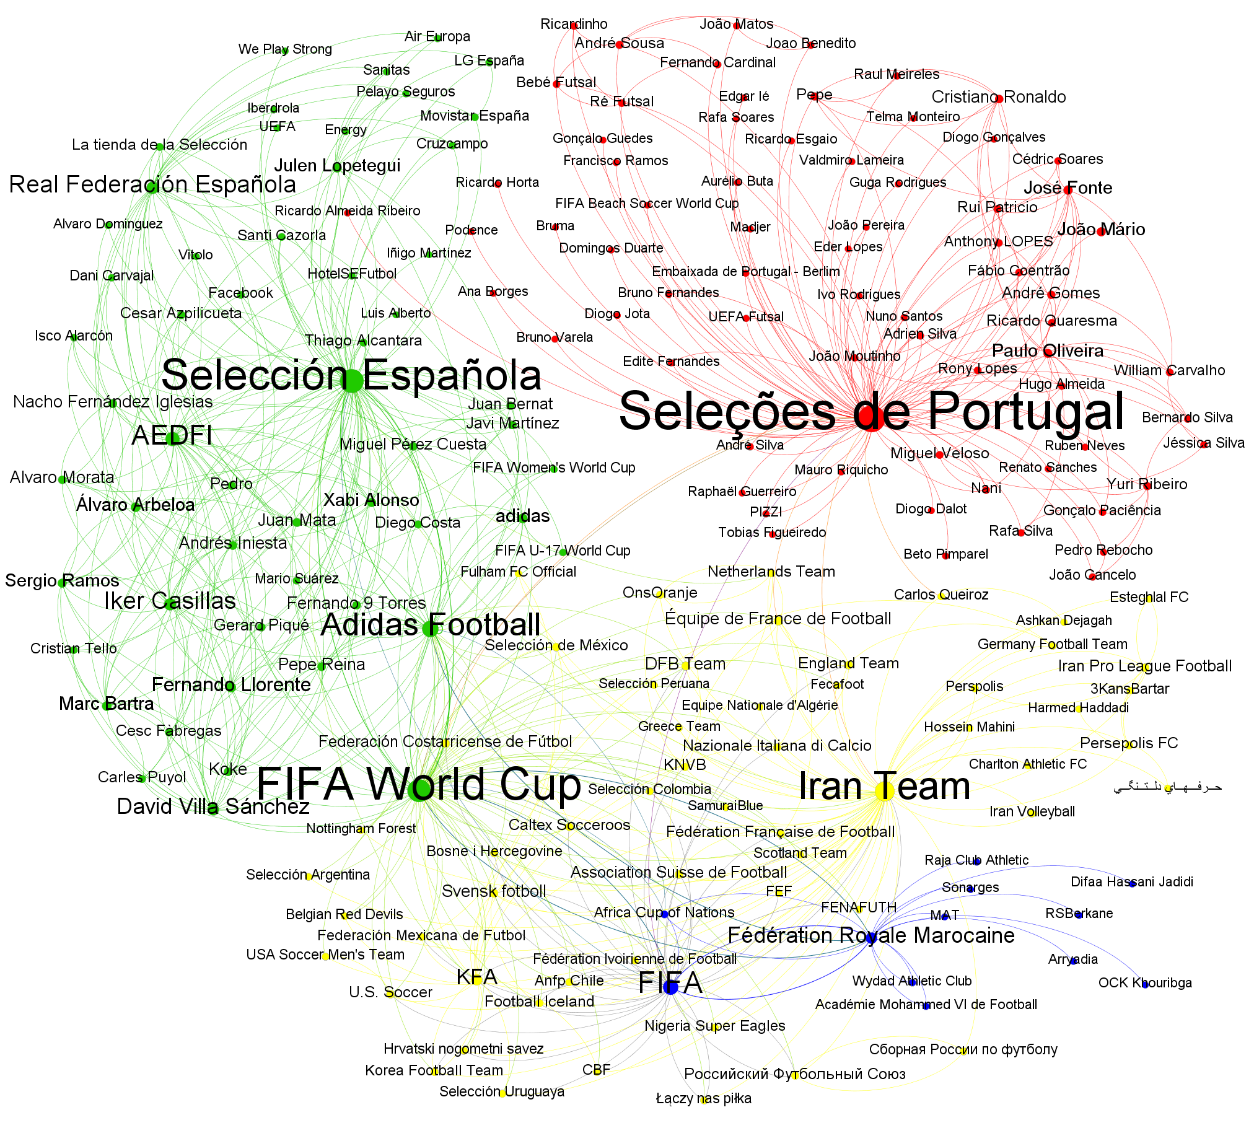
\includegraphics[width=0.85\textwidth]{figure03.png}
 \caption{Grafo de rede das páginas associadas ao Grupo B (n = 194).}
 \label{fig3}
 \source{Facebook Graph API}
\end{figure}
 
O exame do grafo de rede revela ao menos três tendências do Grupo B do Mundial 2018: i) pela proximidade, existe mais interação entre os \emph{stakeholders} vinculados às seleções iraniana, marroquina e espanhola, em oposição ao isolamento dos atores conectados à equipa portuguesa; ii) pela localização, os nós que trabalham como ponte entre as comunidades são outras seleções, entidades reguladoras do futebol e patrocinadores do universo desportivo; iii) pelo tamanho, as páginas têm importância diferente na manutenção da rede, construída em parte pela capacidade de influenciar os outros membros da comunidade e, em alguns casos, as assessorias das equipas nacionais e estrangeiras. Oficialmente, as páginas são geridas em farsi (Irão), árabe (Marrocos), espanhol (Espanha) e português (Portugal), mas é possível encontrar comentários em diferentes idiomas, como inglês, francês ou mandarim.

Com um mundo conectado em rede e a rápida democratização das TIC \cite{castells2009, castells2007}, explorar as tendências de interação entre \emph{stakeholders} parece fundamental para o planeamento de toda e qualquer ação de marketing digital, sobretudo as voltadas ao desporto. Dessa maneira, também é importante mapear, dentro de um grafo, quais atores são mais influentes e o seu perfil diferenciador, principalmente com amostras muito diversas (atletas, equipas, entidades, media, sponsors, governos, etc). O Quadro \ref{tab3} apresenta o ranking dos dez principais influenciadores do Grupo B, com base nas 194 \emph{fanpages} e suas interações na rede. Para tanto foi utilizada a fórmula estatística \emph{Weighted Degree}, no Gephi, que atribui e destaca os mais influentes com auxílio do número de interações \cite{barabasi2016}.

\begin{table}[htpb]
\caption{Ranking dos dez principais influenciadores do Grupo B}
\label{tab3}
\centering
\begin{tabular}{lllll}
\toprule
Colocação & Páginas & Categoria & Seguidores & Weighted Degree
\\
\midrule
1º & Seleções de Portugal & Equipa & 3.726.133 & 104
\\
2º & Selección Española & Equipa & 3.568.061 & 87
\\
3º & FIFA World Cup & Entidade & 40.536.499 & 83
\\
4º & Iran National Team & Equipa & 108.034 & 55
\\
5º & Adidas Football & Sponsor & 28.629.108 & 50
\\
6º & FIFA & Entidade & 3.642.469 & 44
\\
7º & AEdFI & Entidade & 3.115 & 38
\\
8º & Federación Española & Entidade & 469.365 & 28
\\
9º & Iker Casillas & Atleta & 25.138.224 & 28
\\
10º & Fédération Merocaine & Entidade & 276.483 & 24
\\
\bottomrule
\end{tabular}
\centering
\source{Facebook Graph API}
\end{table}
 
Os dados permitem aferir ao menos cinco conclusões sobre os atores mais influentes do Grupo B, entre 1 de abril de 2017 e 3 de maio de 2018:

\begin{enumerate}[label=\roman*.]
\item O TOP 10 é formado por um conjunto muito heterogêneo de \emph{stakeholders} (entidades, atleta, equipas e sponsor) com um alcance potencial variável;
\item A importância da página não é indicada apenas pelo número de seguidores, mas pela capacidade de criar conteúdos percebidos como importantes para a rede. Por exemplo, uma das \emph{fanpages} de maior alcance potencial da rede, a do jogador Cristiano Ronaldo, com mais de 122 milhões de seguidores, não aparece no TOP 10, enquanto a \emph{Asociación Española de Futbolistas Internacionales} (AEdFI), com 3,115 seguidores, está no 7º lugar. Isto ocorre, em grande medida, porque a AEdFI envolveu-se mais com a rede do Grupo B que o futebolista português;
\item Portugal tem a página mais influente da rede, com 104 de \emph{Weighted Degree}, por ser percebida, no ano que antecedeu o Mundial, como produtora de conteúdos importantes para o maior número de nós;
\item Embora o grafo de rede tenha revelado uma diversidade de atores sociais, o TOP 10 é constituído basicamente por organizações do universo desportivo, como FIFA, Iran National Team ou Adidas Football;
\item Apenas um ator humano, o atleta Iker Casilhas, surge no ranking, com 28 de \emph{Weighted Degree}. A explicação provável para esse fenómeno recai nas afiliações desportivas. Casilhas é espanhol, defendia a equipa do seu país e, por isto, estava conectado ao \emph{cluster} de origem (verde, no grafo de rede). Ao mesmo tempo, também era jogador do FC Porto e, por isto, interagia com o \emph{cluster} português (vermelho, no grafo de rede) por intermédio de outros atletas.
\end{enumerate}

Os resultados do quadro permitem identificar os principais influenciadores do Grupo B e as particularidades dessa composição. Porém, os utilizadores de redes sociais passaram a fazer parte dos fluxos de informação e comunicação dos \emph{stakeholders}, enquadrando ou interpretando uma mensagem através dessas plataformas digitais. Por vezes, ampliam a divulgação de versões oficiais, mas também são capazes de resignificar as mensagens, com outros valores associados, para escrever uma narrativa própria. Daí a importância de monitorizar, a longo prazo, o que é dito sobre as marcas, os níveis de interação e a reação dos consumidores em rede. A \cref{fig4} mostra os índices de envolvimento dos fãs com as seleções do Grupo B, mês a mês, com base nas interações em rede (gostos, partilhas, comentários). Para calcular o envolvimento, foi usado a fórmula de \emph{engagement} do Facebook \cite{vadivu2015}.

\begin{figure}[htbp]
 \centering
 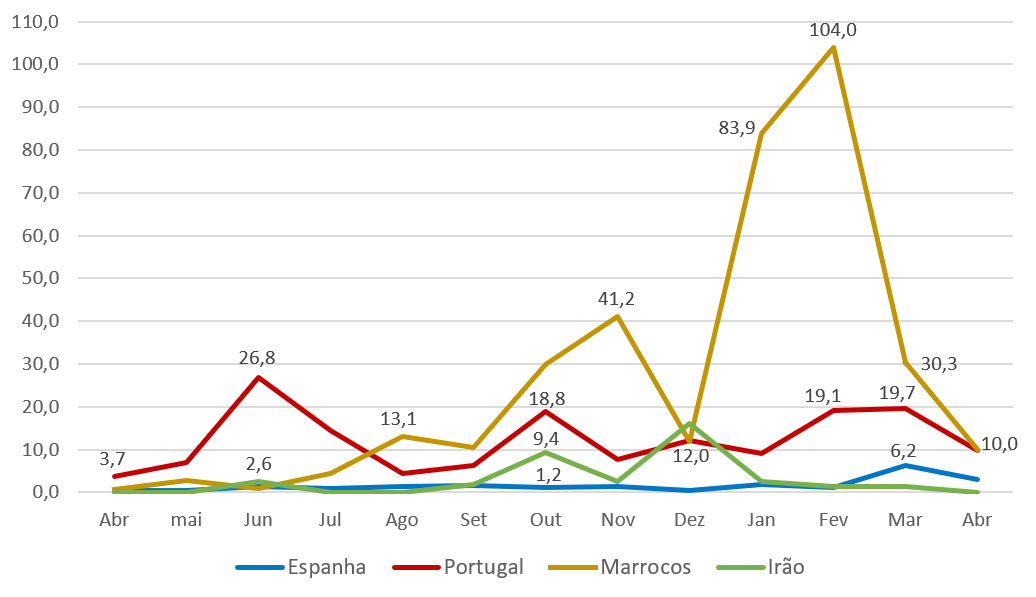
\includegraphics[width=0.7\textwidth]{figure04.png}
 \caption{Envolvimento com as páginas do Grupo B (04/2017 a 04/2018).}
 \label{fig4}
 \source{Facebook Graph API}
\end{figure}

As \emph{fanpages} do Grupo B registaram, no ano analisado, mais de 11 milhões de interações. Portugal, na linha vermelha, apresenta quatro máximas no gráfico: junho de 2017 (participação na Taça das Confederações), outubro de 2017 (apuramento para o Mundial da Rússia, na última partida), fevereiro de 2018 (campeão europeu de futsal) e março de 2018 (duas partidas, contra o Egito e a Holanda). O Irão, na linha verde, tem resultados já esperados ao longo do ano, dados os constrangimentos de acesso à internet no país e o contexto político religioso, com o frequente bloqueio das redes sociais. A única máxima no gráfico, em dezembro de 2017, está relacionada com a publicação de uma sondagem: “O Grupo B é o mais difícil do Mundial?”.

A Espanha, na linha azul, revela um índice baixíssimo de envolvimento, mesmo tendo uma das páginas com o maior número de seguidores do grupo. A única máxima registada, em março de 2018, está diretamente associada à divulgação da lista dos jogadores para o Mundial, e o bom desempenho frente a duas seleções então favoritas ao título: Alemanha e Argentina. Já Marrocos, na linha amarela, possui quatro máximas no gráfico, respectivamente: em novembro de 2017 (apuramento para o Mundial da Rússia, depois de 20 anos de ausência), em janeiro de 2018 (início da campanha para sediar o Mundial de 2026), em fevereiro de 2018 (o clube Wydad A.C. conquista pela primeira vez a Supertaça de África, e é recebido com grande festa no país) e em março de 2018 (apresentação oficial da candidatura para sediar o Mundial).

Em termos anuais, Marrocos lidera graças ao seu desempenho nos primeiros meses de 2018, com o índice médio de 26,4, mas, aparentemente, com crescimento pouco sustentável a longo prazo. Portugal aparece em segundo lugar, com índice de 12,2, na média mais estável do Grupo B. A Espanha ocupa a última posição, com 1,7 de média, atrás até do Irão e seus dilemas internos, com 2,9 pontos.

A partir do cruzamento de dados extraídos do Facebook e do calendário das seleções, é plausível argumentar que esse índice de envolvimento dos fãs nem sempre acompanha os jogos propriamente ditos. Muitas vezes, aparenta oscilar de acordo com os grandes eventos e grandes feitos do país em campo, em uma demonstração de nacionalismo no desporto. Logo, numa das únicas práticas desportivas de alcance global, o apoio ou a rejeição ao desempenho das equipas é também uma espécie de teste de lealdade, estruturado no chauvinismo cultural. Dito por outras palavras, o orgulho de pertencer a um certo povo representado, contra adversários estrangeiros, pelos ‘melhores da espécie’: os atletas de alto rendimento.

Enquanto o futebol desperta a sensação de pertença, no caso do Mundial, fazer parte da saga de um povo também evoca a partilha de sentimentos variados \cite{dorsey2016}. A \Cref{fig5} mostra quais publicações fizeram com que os fãs das seleções mais expressassem amor, a partir da contagem do número de \emph{emojis} desta categoria.

\begin{figure}[htbp]
 \centering
 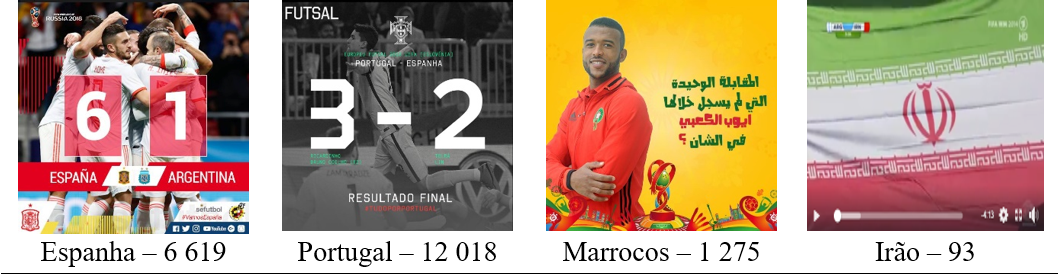
\includegraphics[width=0.85\textwidth]{figure05.png}
 \caption{Publicações que os fãs mais expressaram amor ({\fontspec{Symbola}\symbol{"2764}})}
 \label{fig5}
 \source{Facebook Graph API}
\end{figure}

Os dados mostram a predominância de fotografias, com o Irão sendo única exceção, por publicar um vídeo. Os fãs de Espanha e Portugal celebram o bom desempenho de suas equipas, pela vitória de 6 a 1 sobre a Argentina e a conquista do Campeonato Europeu de Futsal, ocorrido na Eslovênia. Os fãs de Marrocos celebram os feitos de um dos seus jogadores, Ayoub El Kaabi. Os adeptos do Irão expressam amor pelo vídeo que reúne a atuação dos jogadores numa partida difícil; o texto diz, em tradução livre: “Um clip assustador do corajoso jogo da seleção iraniana contra a Argentina. Compartilhe para mostrar solidariedade.” A \Cref{fig6} apresenta as postagens que os fãs mais expressaram raiva.

\begin{figure}[htbp]
 \centering
 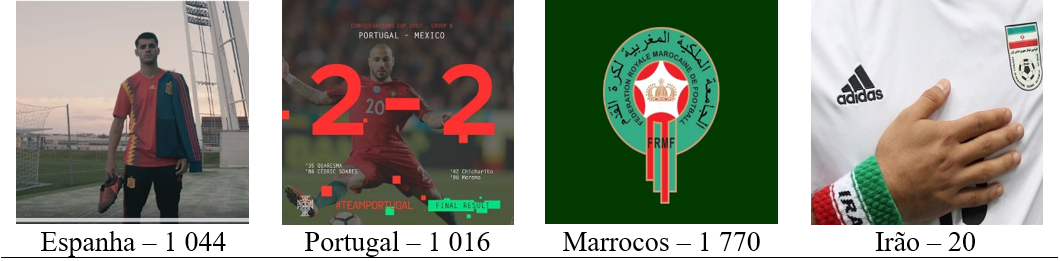
\includegraphics[width=0.85\textwidth]{figure06.png}
 \caption{Publicações que os fãs mais expressaram raiva ({\fontspec{Symbola}\symbol{"1F620}})}
 \label{fig6}
 \source{Facebook Graph API}
\end{figure}

Os resultados revelam a prevalência das imagens, com Espanha sendo a única exceção, por postar um vídeo em \emph{loop}. No caso espanhol, a publicação que mais despertou a ira dos fãs é um apelo à aquisição de um produto; o texto diz, em tradução livre: “Já podes comprar a nossa nova camisola!” Os fãs da Seleção de Portugal irritaram-se com um empate diante do México, por 2 a 2, principalmente porque o golo latino-americano saiu depois dos 90 minutos. No caso marroquino, a raiva voltou-se contra o comunicado do Comitê Disciplinar Central, em que pune o clube do Raja Casablanca pela violência de seus adeptos em um jogo. Os iranianos mostraram mais irritação contra uma publicação relacionada à parceria entre a seleção nacional e a Adidas, em que o pano de fundo são as sanções económicas dos Estados Unidos e a recusa da Nike em vender equipamentos desportivos ao país. A \Cref{fig7} revela as postagens que mais despertaram tristeza nos adeptos.

\begin{figure}[htbp]
 \centering
 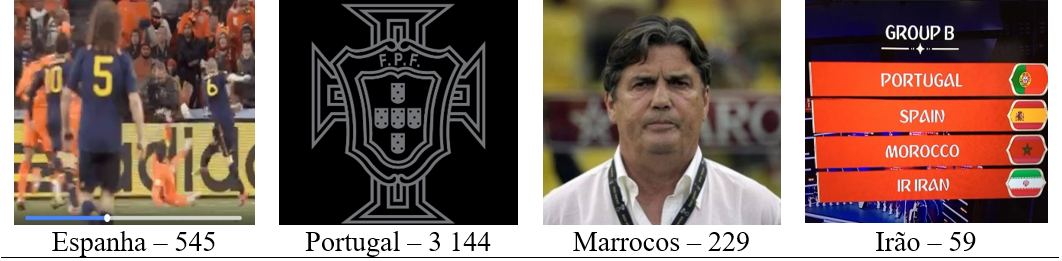
\includegraphics[width=0.85\textwidth]{figure07.png}
 \caption{Publicações que os fãs mais expressaram tristeza ({\fontspec{Symbola}\symbol{"1F613}})}
 \label{fig7}
 \source{Facebook Graph API}
\end{figure}

Os dados indicam a predominância de fotografias, com Espanha sendo a única exceção, por publicar um vídeo. Durante o ano em análise, os fãs espanhóis sentiram-se mais tristes com a despedida de Andrés Iniesta da equipa nacional, considerado um dos melhores marcadores de sempre do país. A publicação que mais comoveu os fãs marroquinos foi o anúncio da morte de Henry Michel, ex-treinador da seleção. Os iranianos lamentaram o resultado do sorteio da FIFA que formou o Grupo B do Mundial, com duas equipas de grande tradição no futebol e a provável eliminação logo na primeira etapa do torneio. A publicação que mais entristeceu os portugueses esteve relacionada aos incêndios florestais na vila de Pedrógão Grande, que resultaram na morte de 66 pessoas; o texto diz: “O dia em que iniciamos a participação na Taça das Confederações é igualmente um dia de grande dor para o País que orgulhosamente representamos”.

\section{Conclusões: muito além do relvado}\label{sec-conclusoes}
A partir de complexas dinâmicas da globalização \cite{giddens1999}, é possível destacar a relevância do desporto enquanto prática eminentemente cultural e identitária, tal como o seu incontornável papel na intensificação das relações, unindo e separando povos à escala global. Este artigo revelou que as mais de 11 milhões de interações analisadas (gostos, partilhas, \emph{emojis}, comentários) estão associadas, geralmente, ao orgulho diante dos grandes eventos e dos grandes feitos do país frente aos adversários estrangeiros.

Certo é que, a par de outras esferas da vida em sociedade, o desporto e, em particular, o futebol, passam por profundas convulsões nas últimas décadas, sendo o impacto das tecnologias uma das mais reveladoras \cite{castells2007, castells2009}. É possível notar, a partir das publicações analisadas, uma tentativa de não apenas melhorar a experiência dos fãs, mas também potenciar o seu papel cocriativo, tornando-os membros ativos na organização, na produção e no consumo dos eventos. Assim, estariam embrenhados em uma cultura de participação de todos para todos. De olhos postos no Mundial 2018, fica evidente que as redes sociais, em especial o Facebook, são uma fonte agregadora e confiável de informações para os adeptos.

Ao navegarem pela rede social, os fãs de futebol, ao mesmo tempo que contribuem para a edificação de uma comunidade global, o seu acesso, os modos e a frequência como interagem são condicionados pelo contexto económico, tecnológico e político offline. Tais forças também determinam, em grande medida, os fluxos informativos e paradigmas comunicacionais de cada país. É importante pensar que uma leitura pós-colonial também indicaria outros condicionantes mais presentes no Irão e Marrocos que em Espanha e Portugal. Em larga medida, essas forças tendem a moldar os fluxos comunicacionais, o acesso às infraestruturas tecnológicas e as formas de participação política \cite{hobsbawm2003, kamrava2012}. No fundo, cada contexto é resultado do seu longo e tortuoso processo histórico.

Do estudo das interações entre os diferentes \emph{stakeholders}, é possível argumentar que a relevância das páginas não deve ser aferida só pelo número de seguidores. É preciso considerar a capacidade de criar conteúdos percebidos como relevantes para gerar envolvimento dentro da rede. Nesse caso, a \emph{fanpage} da seleção portuguesa se destaca como a mais importante do Grupo B, sendo percecionada como a principal produtora de conteúdos capazes de impactar diferentes \emph{stakeholders} (entidades, atletas, equipas, sponsors). De resto, um dado curioso advém do fato de, num universo onde se destacam as celebridades individuais, arrastando consigo milhões de fãs, predominarem como influenciadores as páginas de organizações e de entidades desportivas. Esse dado é ainda mais interessante tendo em conta que muitas das contas com mais seguidores, no Facebook, pertencem justamente a jogadores \cite{clavio2010}.

A análise de sentimentos via \emph{emojis} mostra que, como num jogo de futebol, os adeptos reagem com amor, raiva ou tristeza à predominância das publicações fotográficas no Facebook. Contudo, tal expressão não verbal das emoções \cite{novak2015} nem sempre acompanha o que se passa dentro das quatro linhas. O índice de envolvimento dos fãs também oscila em razão de questões nacionais prementes da agenda social, económica e política. Esse fenômeno é claro quando observados os incêndios florestais na vila de Pedrógão Grande, em Portugal, ou a recusa da Nike em vender equipamentos a um país sob o embargo norte-americano, como no caso do Irão. Em ambos os exemplos, há questões estruturantes da identidade nacional que não estão diretamente associadas ao culto à bola.

Como qualquer investigação, há limitações que estudos vindouros podem colmatar. Em primeiro lugar, as recentes mudanças nas políticas de acesso à API do Facebook fazem com que se torne cada vez mais complexo recolher informações, desta rede, que possam ser tratadas como Big Data. Depois, como atletas, entidades e seleções tendem a trabalhar como diferentes plataformas, os dados de uma única rede social apresentam um retrato provisório da atuação dos \emph{stakeholders}. Por fim, estudos futuros precisam considerar as particularidades de cada rede social, como Twitter, Instagram e YouTube, para definir os métodos de recolha de informações mais apropriados. Como já é sabido \cite{ahn2014}, cada plataforma influencia o tempo de uso por parte dos fãs do desporto.




\printbibliography\label{sec-bib}
% if the text is not in Portuguese, it might be necessary to use the code below instead to print the correct ABNT abbreviations [s.n.], [s.l.] 
%\begin{portuguese}
%\printbibliography[title={Bibliography}]
%\end{portuguese}

%full list: conceptualization,datacuration,formalanalysis,funding,investigation,methodology,projadm,resources,software,supervision,validation,visualization,writing,review
\begin{contributors}[sec-contributors]
\authorcontribution{Branco Di Fátima}[conceptualization,datacuration,formalanalysis,investigation,visualization,writing,review]
\authorcontribution{Célia Gouveia}[conceptualization,formalanalysis,investigation,methodology,writing]
\authorcontribution{Sandra Miranda}[methodology,supervision,validation,review]
\end{contributors}


\end{document}
